\section{Datasets}

In this section all datasets are described that are used in this work.
The first subsection describes which subsets of RailSem19 are used for the first attempt for the training of object detection models.
Then the annotations of \cite{tepNet2024} are briefly discussed, which are used to train all single-frame-based models.
After that a switch evaluation dataset is described that is used to evaluate singe-frame models on switch scenarios.
The last subsection deals with the temporal dataset and its creation.


\subsection{RailSem19 and subsets for training object detection models}

The first approach to creating a Rail Track Prediction system includes combining an object detection model with a semantic segmentation model.
Since RailSem19 supports both of these methods this dataset is chosen for training.
Furthermore, state-of-the-art research in \autoref{sec:datasets} shows that this dataset is the only one that not only includes switch annotations but also labels for switch states: $switch\_left$, $switch\_right$.
Since not all states are identifiable even though a switch is visible there also is the $switch\_unknwon$ label.

In this work, the bounding boxes are utilized to train the \ac{YOLO} object detection models.
Experiments have been conducted with three versions of this dataset.
An overview of these subsets is shown in \autoref{tab:usedSubsetsforYOLOs}.
The first set is the whole dataset, which includes 8500 images with all different bounding box labels.
The second subset only considers images with switch labels including the $switch\_unknown$ label.
For this subset, 2764 images remain. The third subset only considers the switch labels in which the state is identifiable.
This is because when focusing on the train's direction, the $switch\_unknown$ label does not hold any valuable information.
To prevent confusion, all images containing $switch\_unknown$ annotations are intentionally excluded, resulting in a final set of 1,240 images.

\begin{table}[H]
    \centering
    \begin{tabular}{|l|l|l|}
    %\begin{tabular}{| p{0.3\linewidth} | p{0.6\linewidth} |}
        \hline
        \textbf{RailSem19} & \textbf{RailSem19\_onlySwitches} & \textbf{RailSem19\_onlySwitchesLeftRight}\\
        \hline
        8500 images & 2764 images & 1240 images\\
        \hline
        all bounding box labels & $switch\_left$ & $switch\_left$\\
        \hline
        & $switch\_right$ & $switch\_right$\\
        \hline
        & $switch\_unknown$ & images with $switch\_unknown$ excluded\\
        \hline
    \end{tabular}
    \caption{Used dataset subsets of RailSem19 for training \ac{YOLO} object detection models}
    \label{tab:usedSubsetsforYOLOs}
\end{table}

Since the experiments of training object detection models showed unsatisfactory results also described in <section>, this methodology was deemed ineffective.
This leads to the pursuit of a different solution and experiments with semantic segmentation models are therefore not accomplished.
Consequently the corresponding dense labels of the RailSem19 dataset are not utilized.

\clearpage
\subsection{TEP annotations}

For training single-frame-based models \cite{tepNet2024} published its annotations for the images of RailSem19.
These annotations consist of polylines for the left and the right rail of the train.
Only the two rails are included in the labels which the train drives on.
This is also the case when switches are present.
Additionally, some images are excluded from this dataset when the train's track is not identifiable.
For labeling this dataset the online tool CVAT \cite{cvat} is used.
These annotations can then be transformed with pre processing step to support other models like semantic segmentation. 
This dataset is described in more detail in \autoref{subsubsec:TEP-Net_dataset}.

\subsection{Switch evaluation dataset}

For a practical application, it is important to make the output as useful and visible as possible.
Therefore, the output should be the whole track, not only the rails.
This is realized in the post-processing by filling out the area between the rails resulting in a binary mask.
This mask is similar to the output of semantic segmentation techniques.
It gives each pixel either the class label $track$ or $no\_track$.
For these methods, the most common evaluation metric is the \ac{IoU}, which is also used by \cite{tepNet2024} to evaluate models on the test set.

This metric has its justification for general rail track prediction scenarios because it is a good indicator of model performance.
However, when switches are present in the scene the \ac{IoU} often loses meaningfulness.
This issue is visualized in \autoref{fig:incorrectButHighIoU}.
In this example, the model cannot correctly predict the train's path at the switch.
Contrary to this uncertainty, the \ac{IoU} still gives a high value indicating a good performance even though the direction of the train is wrong.
The reason for this lies in the calculation of the \ac{IoU} and this specific problem case.
Since the switch is in the distance and the track is mostly correct up to this point, the predicted mask and the mask of the \ac{GT} still share a great portion of their areas.
This leads to high values of the \ac{IoU} metric, even though the track is incorrect.

\begin{figure} [H]
    \centering
    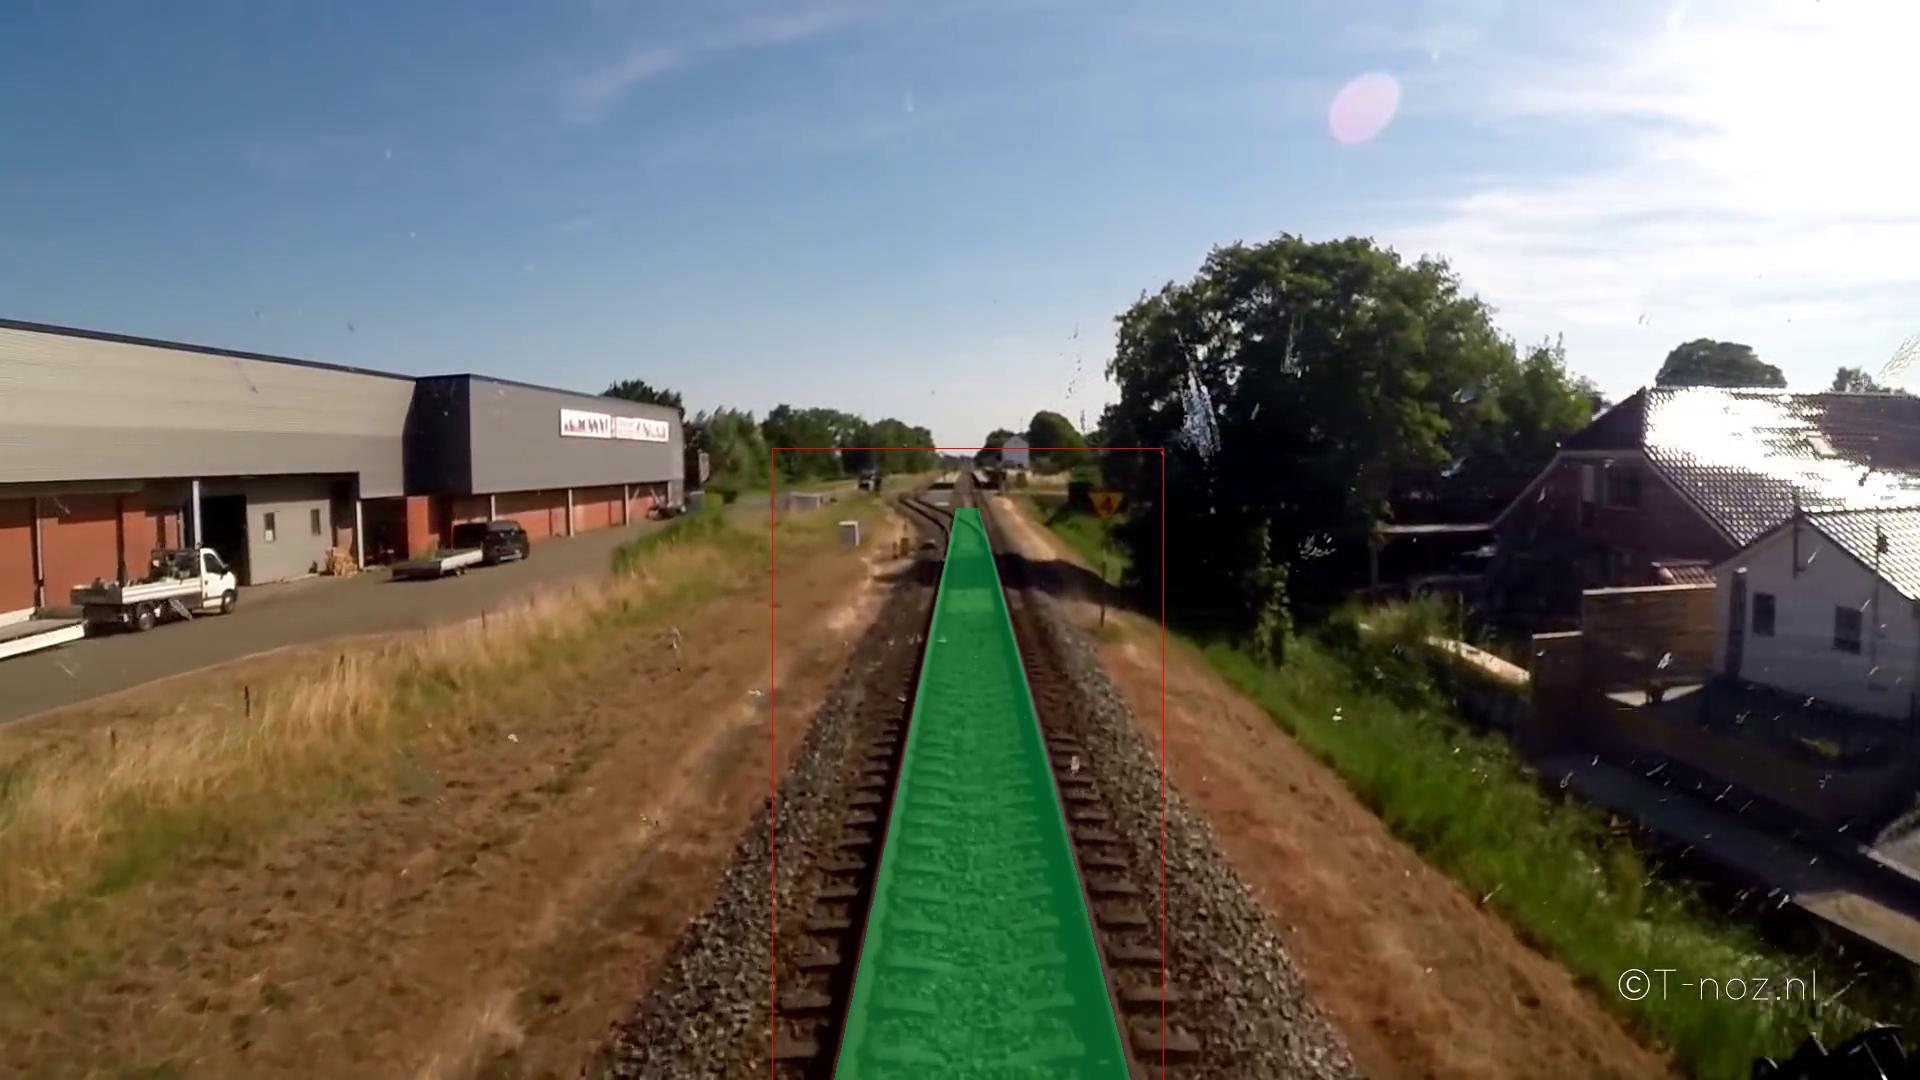
\includegraphics[width=0.7\linewidth]{PICs//usedDatasets/falsch_aber_hohe_IoU.jpg}
    \caption{Example of a switch scene that is incorrectly predicted, but the \ac{IoU} metric still returns high values presenting potentially misleading performance scores. Track continuous to the left.}
    \label{fig:incorrectButHighIoU}
\end{figure}

Since this work especially focuses on correctly predicting the train's direction in scenarios with switches, a solution to this evaluation issue must be found.
Therefore a switch evaluation dataset is created, which solely focuses on switch scenarios.
Furthermore, a points system is created that gives insight into the model performance.
This point system is shown in <Figure xy>.
The dataset consists of all images that contain switch cases out of the validation and test dataset that are obtained from the $80\%-10\%-10\%$ split of \cite{tepNet2024}.
This results in 67 images which include 72 switches in total.
The model gets 1 point for each correctly predicted switch.
There are cases where models correctly filter out the track and set the horizon line before the switch.
This behavior is rewarded with 0,5 points.
This behavior is assumed to come from the labeling policy with $switch\_unknown$ labels.
In \cite{tepNet2024} in images with $switch\_unknown$ labels, the track is annotated up to this label.
This shows that the model is uncertain about the switch state.
However, setting the horizon line before the switch is preferred over predicting the track incorrectly.
In other cases, the model does not get any points.

\begin{figure}[H]
    \centering
    \begin{subfigure}[b]{0.48\textwidth}
        \centering
        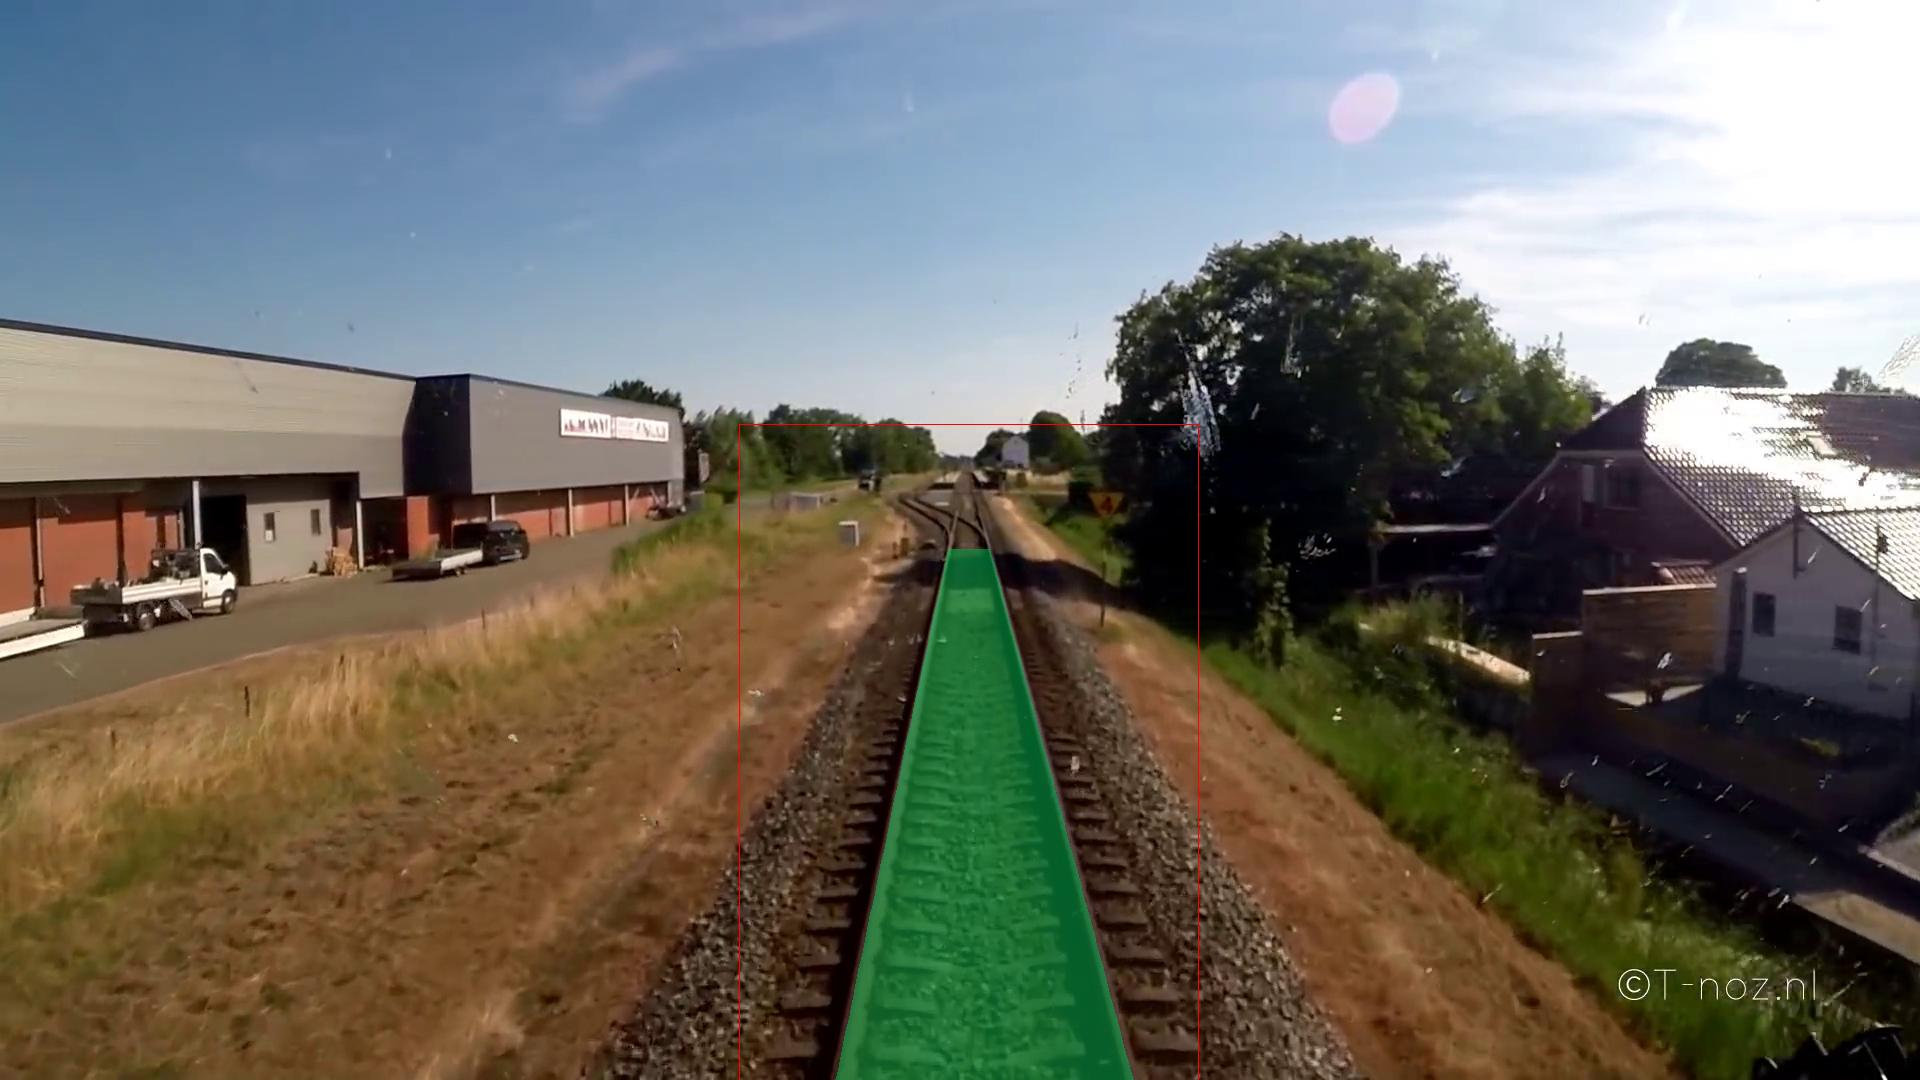
\includegraphics[width=\textwidth]{PICs/usedDatasets/0,5punkte.jpg}
        \caption{0.5 points}
    \end{subfigure}
    \hfill
    \begin{subfigure}[b]{0.48\textwidth}
        \centering
        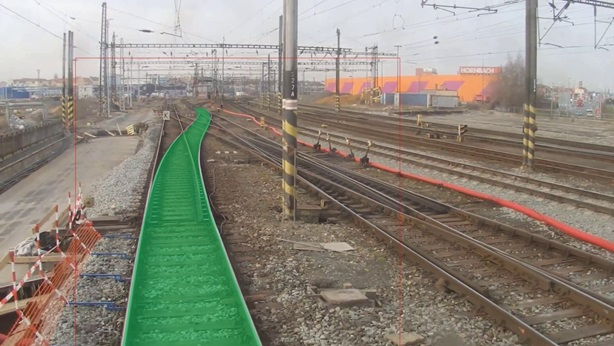
\includegraphics[width=\textwidth]{PICs/usedDatasets/1punkt.jpg}
        \caption{1 point}
    \end{subfigure}
    
    \vspace{0.5cm} % Abstand zwischen den Zeilen

    \begin{subfigure}[b]{0.48\textwidth}
        \centering
        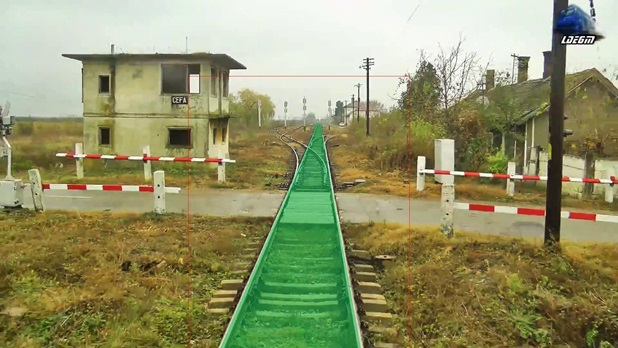
\includegraphics[width=\textwidth]{PICs/usedDatasets/2punkte.jpg}
        \caption{2 points (2 switches)}
    \end{subfigure}
    \hfill
    \begin{subfigure}[b]{0.48\textwidth}
        \centering
        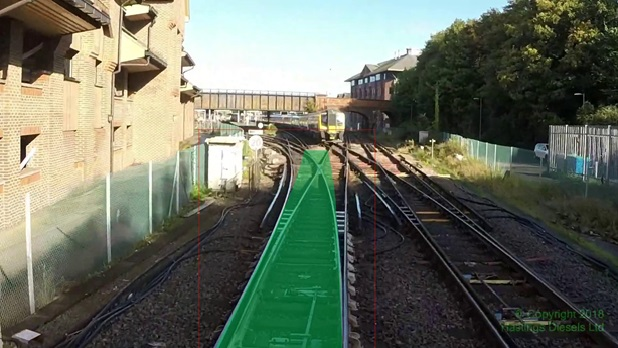
\includegraphics[width=\textwidth]{PICs/usedDatasets/0punkte.jpg}
        \caption{0 points}
    \end{subfigure}
    \caption{Scoring system of the switch evaluation dataset.}
    \label{fig:pointSystem}
\end{figure}

This switch dataset deals with a qualitative performance evaluation and no technique is found to automate this process.
Therefore, a model predicts the track of each image, and the points are given by manually observing outputs.
Since the prediction process should resemble a real application, the autocrop technique is utilized.
By predicting each image 50 times crop coordinates have time to converge to a crop similar to one in real applications.

\subsection{Temporal Dataset}

To train temporal models a dataset must be used that consists of videos and not only single images.
\cite{tepNet2024} stated that there is no public temporal dataset available for the rail domain, which can be used for this use case.
This statement is correct, to the best of the authors knowledge.
Therefore a YouTube video \cite{temporalDataset_youtube_video} from the RailSem19 dataset is used.
No frames that are used in the RailSem19 dataset are used in the proposed temporal dataset.
Since the focus on the problem formulation of all temporal models is to improve the performance when driving over switches, the new dataset consists of short sequences dealing with this exact used case.
All seconds in the video \cite{temporalDataset_youtube_video} are marked in which the train is located over a switch.
Frames before and after these marked seconds are saved, resulting in 38 sequences with 76 frames each. These are annotated like the dataset used to train single-frame models.

Labeling 2888 images is very time-intensive and repetitive.
Therefore, an auto-labeling strategy is implemented.
The best-performing single-frame-based model in combination with the adapted auto-crop method is utilized.
Each image is processed 50 times so the auto-crop coordinates can adapt and only the most relevant region is considered.
<Figure xy> shows the process from this point.
First, the mask's borders are taken, and then the horizon line is deleted leaving the lines of the rails.
Only two pixels remain in each row as visualized in <Figure xy b>.
These represent the final polylines. To minimize data only every fifth point is saved.
This results in polylines consisting of roughly 62 points, which is the average number of points used to build polylines in the original dataset.
Not all frames are correctly labeled because the temporal dataset focuses on scenes where the single-frame model is bound to fail.
All incorrect annotated images are therefore manually edited in CVAT \cite{cvat}.

\begin{figure}[H]
    \centering
    \begin{subfigure}{0.3\textwidth}
        \centering
        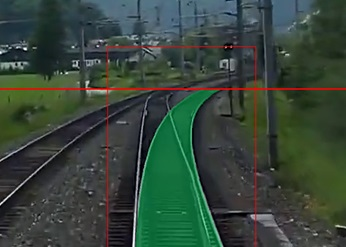
\includegraphics[width=\linewidth,height=5cm,keepaspectratio]{PICs/usedDatasets/predictedImage.jpg}
        \caption{}
        \label{fig:autolabler_a}
    \end{subfigure}
    \hspace*{0.02\textwidth} % Abstand manuell steuern
    \begin{subfigure}{0.3\textwidth}
        \centering
        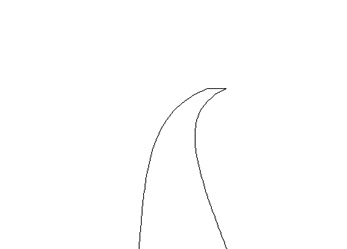
\includegraphics[width=\linewidth,height=5cm,keepaspectratio]{PICs/usedDatasets/maskBorders.jpg}
        \caption{}
        \label{fig:autolabler_b}
    \end{subfigure}
    \hspace*{0.02\textwidth} % Abstand manuell steuern
    \begin{subfigure}{0.3\textwidth}
        \centering
        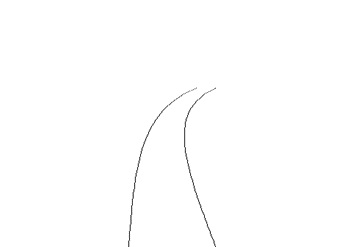
\includegraphics[width=\linewidth,height=5cm,keepaspectratio]{PICs/usedDatasets/justLines.jpg}
        \caption{}
        \label{fig:autolabler_c}
    \end{subfigure}
    \caption{Process steps of auto-labeling: \textbf{(a)} prediction of best single-frame model and autocrop with 50 interations, \textbf{(b)} borders of prediction mask, \textbf{(c)} droped horizon line resulting in auto labeled polylines. All images are zoomed in for better visualization.}
    \label{fig:autolabler}
\end{figure}